%%%%%%%%%%%%%%%%%%%%%%%%%%%%%%%%%%%%%%%%%%%%%%%%%%%%%%%%%%%%%%%%%%%%%%
%%                    Interaction
%%%%%%%%%%%%%%%%%%%%%%%%%%%%%%%%%%%%%%%%%%%%%%%%%%%%%%%%%%%%%%%%%%%%%%
%\color{blue}

\subsubsection{Glyph: \glyph{Interaction}}\label{sec:interaction}

\glyph{Interaction} represents an interaction between two or more \glyph{entities} or \glyph{outcomes}, whether a non-covalent physical interaction, or a functional interaction, e.g. genetic interaction. Each arrowhead points to an interactor involved in the interaction. The result of the interaction is represented by \glyph{outcomes} (see section \ref{sec:outcome}), that is by filled dots on the line linking the two arrowheads in the case of a binary interaction, on a circle linked to the edges coming from the arrowheads in the case of a  n-ary interactions. The result of an interaction can be represented by any number of \glyph{outcomes}.

\begin{glyphDescription}
 \glyphSboTerm SBO:0000342 molecular or genetic interaction
 \glyphOrigin Any \glyph{interactor} (\sect{interactors}).
 \glyphTarget Any \glyph{interactor} (\sect{interactors}).
 \glyphEndPoint Both origin and target extremities of an \glyph{interaction} carry an harpoon arrowhead. In the case of n-ary interactions, the arrows pointing to the \glyph{interactors} originate from a circle. 
\glyphAux A \glyph{unit of information} containing a \glyph{cardinality} (\sect{miscellaneous-cv}) indicates the number of instances of an entity involved in an interaction. The absence of a \glyph{cardinality} is synonymous of a cardinality of 1. A \glyph{unit of information} on a binary interaction involving only one entity carrying the mention \glyph{cis} or \glyph{trans} precises if the interaction is intra-molecular or between different instances of the same entity.
 \end{glyphDescription}

\begin{figure}[H]
  \centering
  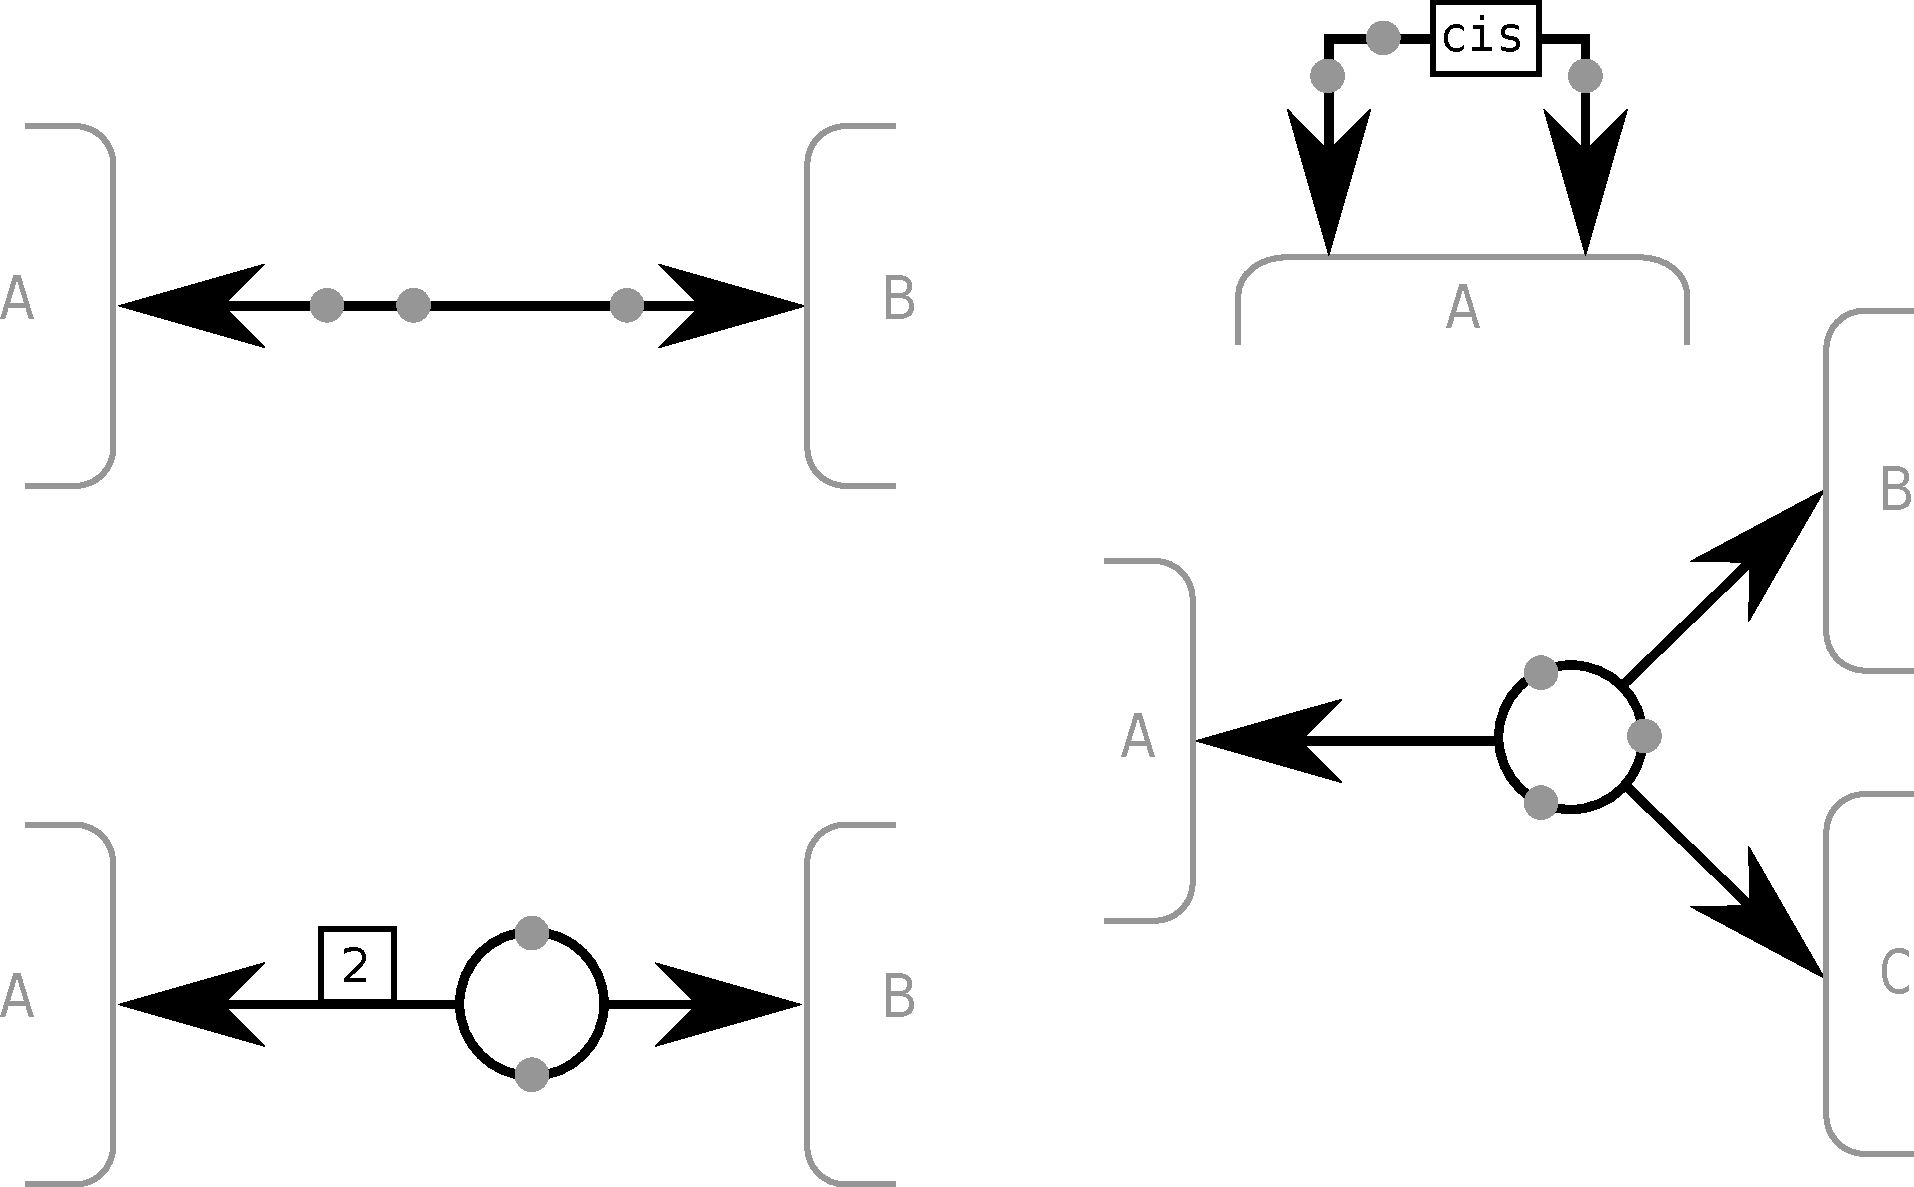
\includegraphics[scale = 0.3]{images/interaction}
  \caption{The \ER glyph for \glyph{interaction}. Top left, binary interaction between two entities. The circle can be ommitted, and the \glyph{outcomes} located anywhere on the \glyph{interaction}. Bottom left, because the cardinality of the entity A is 2, the interaction is not a binary one, but a n-ary one. The circle cannot be ommitted. Bottom right, n-ary interaction with three different entities. Top right, intra-molecular interaction; }
  \label{fig:interaction}
\end{figure}

\begin{figure}[H]
  \centering
  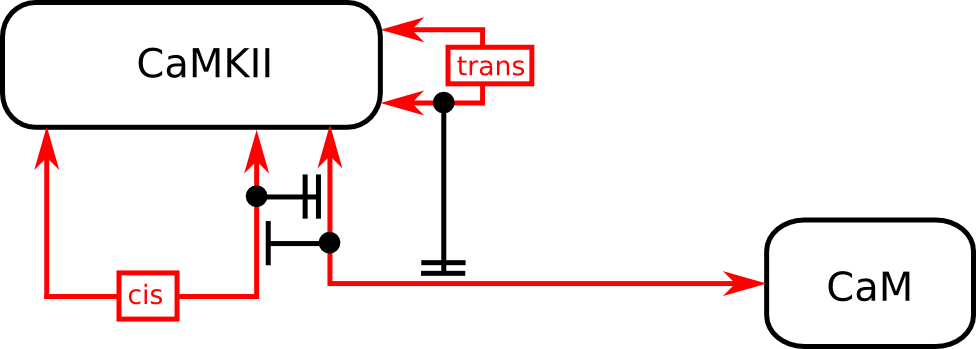
\includegraphics[scale = 0.5]{examples/ex-interaction}
  \caption{Examples of \glyph{interactions}, showing the effect of the binding of calmodulin to CaMKII (binary interaction) on the folding of the kinase (intra-molecular interaction), and the effect of the folding or the dimerisation of CaMKII (inter-molecular interaction between different instances of CaMKII) on the binding of calmodulin.}
  \label{fig:ex-interaction}
\end{figure}


%\normalcolor